\documentclass[conference]{IEEEtran}
\IEEEoverridecommandlockouts
\usepackage{cite}
\usepackage{amsmath,amssymb,amsfonts}
\usepackage{algorithmic}
\usepackage{graphicx}
\usepackage{textcomp}
\usepackage{xcolor}
\usepackage{lipsum}
\usepackage{blindtext}
\usepackage{subfig}
\usepackage{caption}
\usepackage{placeins}
\usepackage{afterpage}
\graphicspath{{./images/}}

\def\BibTeX{{\rm B\kern-.05em{\sc i\kern-.025em b}\kern-.08em
    T\kern-.1667em\lower.7ex\hbox{E}\kern-.125emX}}

\begin{document}

\title{Deep Reinforcement Learning with the MuJoCo Physics Simulator}

\author{
    \IEEEauthorblockN{Curtis Brinker}
    \IEEEauthorblockA{cjbzfd@mst.edu}
    \and
    \IEEEauthorblockN{Tanner May}
    \IEEEauthorblockA{tmay@mst.edu}
}
\maketitle

\begin{abstract}
    \blindtext
\end{abstract}

\section{Introduction}

Recent developments in machine learning have made huge strides in approaching problems that were previously unsolvable
with traditional programming methods. In general, machine learning techniques are grouped into three categories:
supervised learning, unsupervised learning, and reinforcement learning (RL). \cite{rl_application}

\blindtext
\blinditemize[4]

\blindtext

\section{Testing Environment}

Each of the models were trained using Open AI's Gym library and DeepMind's physics simulator MuJoCo on the Ubuntu
operating system with Python 3.8. The Gym toolkit implements numerous environments for testing RL, such as the MuJoCo
physics simulator. MuJoCo stands for {\bf Mu}lti-{\bf Jo}int dynamics with {\bf Co}ntact and was made for applications
that require fast, accurate physics simulations such as robotics and machine learning [Citation from MuJoCo docs]. Using
MuJoCo, machine learning algorithms can learn how to control the movement of robotic models, such as a snake, ant, or
humanoid.

Each of Gym's environments adhere to a strict structure that makes it easy to switch testing environments. One of the
most important parts to keep consistent is the values returned after every step of training [Citation from Gym docs for the following list]:

\begin{itemize}
    \item Observation: Represents the current state of the environment, as the agent sees it. In MuJoCo's case, the
    environment is fully observable and consists of the model's position, velocity, and various forces [citation from humanoid v3 source]
    \item Reward: The reward result of the previous action. The reward for the MuJoCo environment is quite simple: if
    the simulation is still running, give a reward.
    \item Done: A flag denoting if the environment needs to be reset. Each of the models in MuJoCo define a safe height
    range that the model is allowed to exist within; if the model leaves that range, the done flag is raised and the
    model is reset back to the start.
    \item Info: Some information useful for debugging.
\end{itemize}

\section{Background}

\blindtext

\subsection{Advantage Actor Critic (A2C)}

\blindtext

\subsection{Deep Deterministic Policy Gradient (DDPG)}

\blindtext

\subsection{Soft Actor Critic (SAC)}

\blindtext

\section{Methodology}



\section{Results}

\blindtext

\subsection{CartPole-v0}

\blindtext

\subsection{Pendulum-v1}

\begin{figure}
    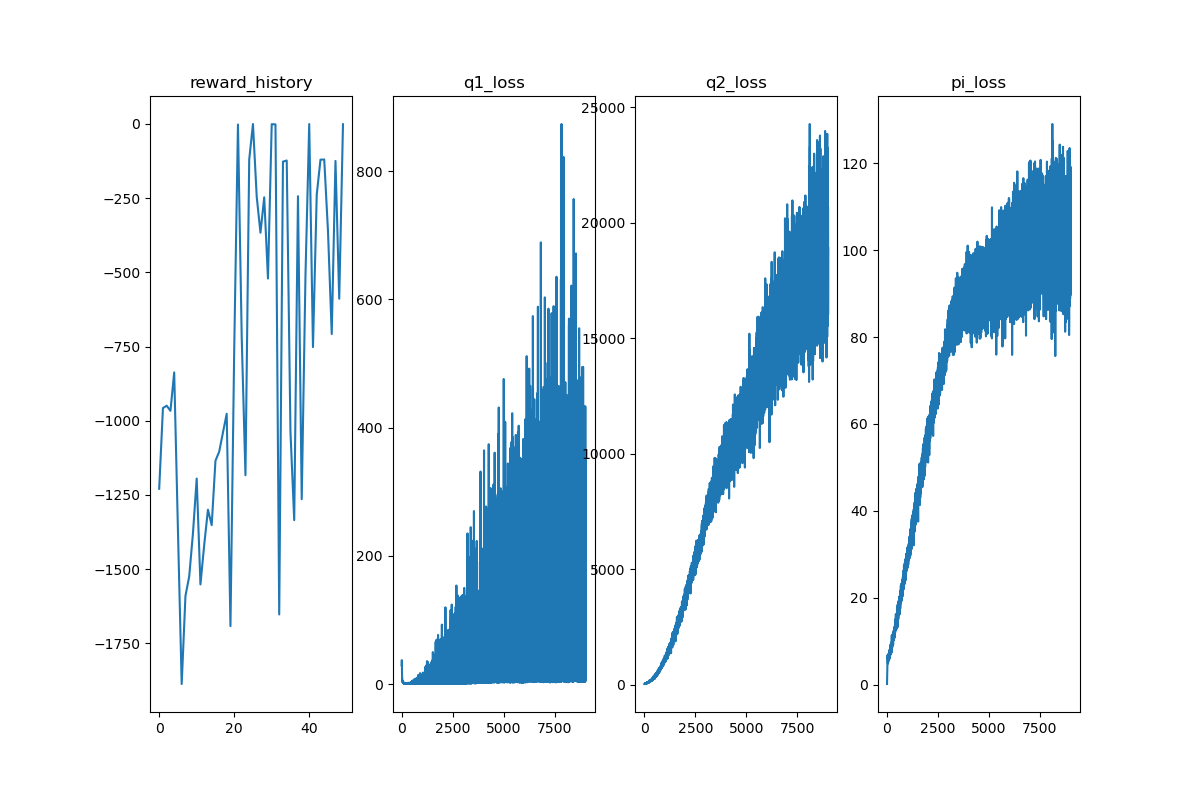
\includegraphics[width=0.45\textwidth]{sac-pendulum}
    \caption{SAC in the Pendulum-v1 Environment}
\end{figure}

\blindtext

\subsection{Ant-v3}

\begin{figure}
    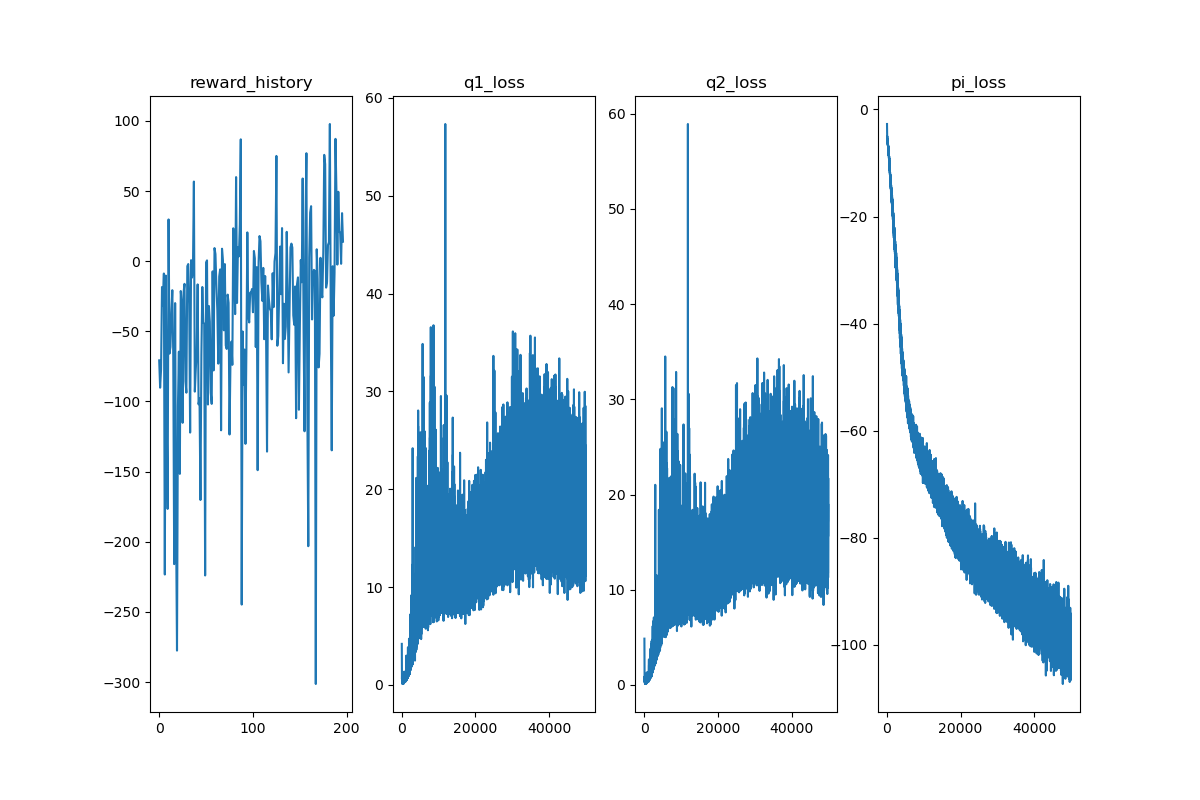
\includegraphics[width=0.45\textwidth, height=5cm]{sac-ant}
    \caption{SAC in the Ant-v3 environment}
\end{figure}

\begin{figure}
    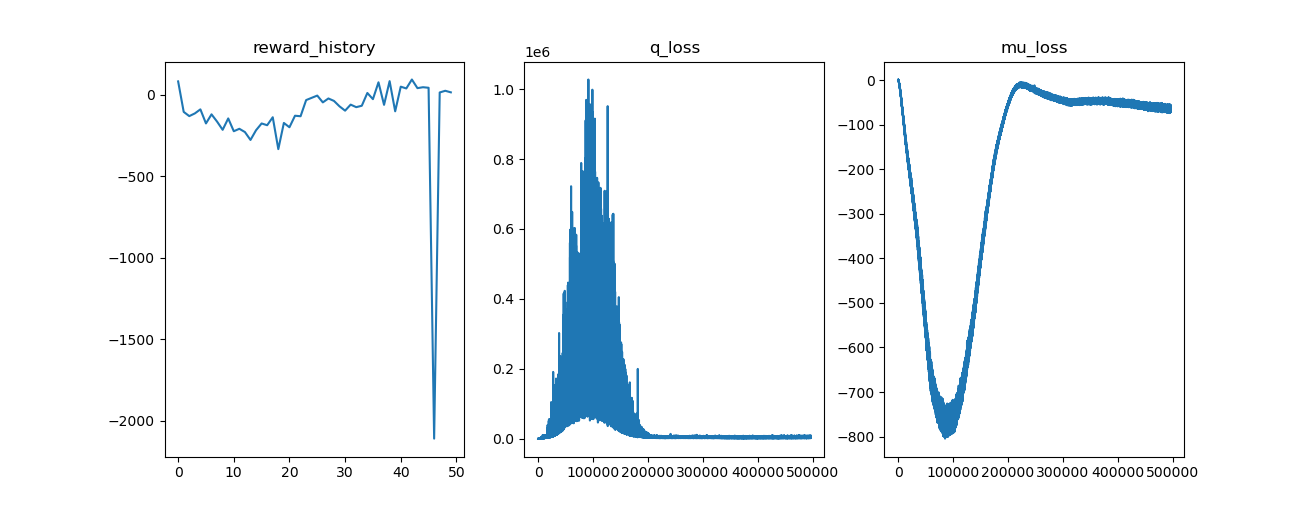
\includegraphics[width=0.45\textwidth, height=5cm]{ddpg-ant}
    \caption{DDPG in the Ant-v3 environment}
\end{figure}

\blindtext

\subsection{Humanoid-v3}

\blindtext

\section{Future Work and Conclusions}

\blindtext[2]


\bibliography{references}
\bibliographystyle{ieeetran}


\end{document}
